%
% $Id: $
%
%
% Compilar a .pdf con LaTeX (pdflatex)
% Es necesario instalar Beamer (paquete latex-beamer en Debian)
%

%
% Gr�ficos:
% Los gr�ficos pueden suministrarse en PNG, JPG, TIF, PDF, MPS
% Los EPS deben convertirse a PDF (usar epstopdf)
%

\documentclass{beamer}
\usetheme{AnnArbor}
%\usebackgroundtemplate{\includegraphics[width=\paperwidth]{format/libresoft-bg.png}}
%\usepackage[spanish]{babel}
\usepackage[latin1]{inputenc}
\usepackage{graphics}
\usepackage{amssymb} % Simbolos matematicos
\usepackage{url}
\usepackage{multirow}
\usepackage{subfigure}

\addtobeamertemplate{navigation symbols}{}{%
    \usebeamerfont{footline}%
    \usebeamercolor[fg]{footline}%
    \hspace{1em}%
    \insertframenumber/\inserttotalframenumber
}


%\definecolor{libresoftgreen}{RGB}{162,190,43}
%\definecolor{libresoftblue}{RGB}{0,98,143}

%\setbeamercolor{titlelike}{bg=libresoftgreen}

%% Metadatos del PDF.
\hypersetup{
  pdftitle={Welcome to SoHeal 2018},
  pdfauthor={Bram Adams, Eleni Constantinou, Tom Mens, Gregorio Robles},
  pdfcreator={Gregorio Robles},
  pdfproducer=PDFLaTeX,
  pdfsubject={Welcome to SoHeal 2018},
}
%%

\begin{document}

\title{Welcome to SoHeal 2018}
\subtitle{1\textsuperscript{st} International Workshop on Software Health}
\institute{}
\author[]{}
\date{Gothenburg, May 27\textsuperscript{th} 2018}


%\AtBeginSection{\frame{\sectionpage}}

\frame{
\maketitle
\begin{center}
\vspace{-1cm}
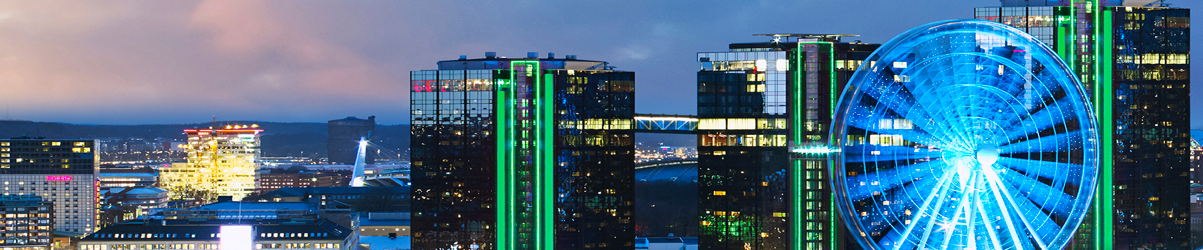
\includegraphics[width=10cm]{figs/gothenburg.png}

\end{center}
}


%%--------------------------------------------------------

\section{\#soheal18}


%-----------------------    ---------------------------------

\begin{frame}
\frametitle{Welcome}

\begin{center}
\Huge Welcome to Gothenburg!
\end{center}


\end{frame}

\usebackgroundtemplate{}


%-----------------------    ---------------------------------

\begin{frame}
\frametitle{Organizing Committee}

\begin{center}
	\begin{figure}[t!]
		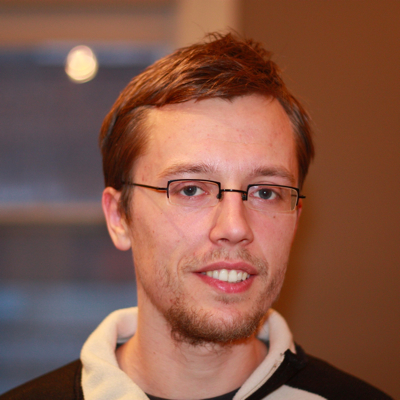
\includegraphics[width=2cm]{figs/bram}
		\hspace{1.6cm}
		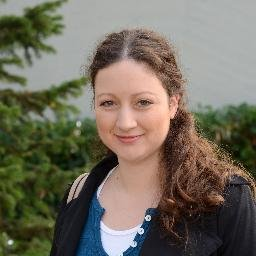
\includegraphics[width=2cm]{figs/eleni}    
		\\ \hspace{0.3cm} Bram Adams \hspace{1cm} Eleni Constantinou
		\vspace{0.1cm}
		\\ Polytechnique Montreal \hspace{0.6cm} Univ. Mons \hspace{0.9cm}
	\end{figure}
\end{center}

\begin{center}
	\begin{figure}[t!]
		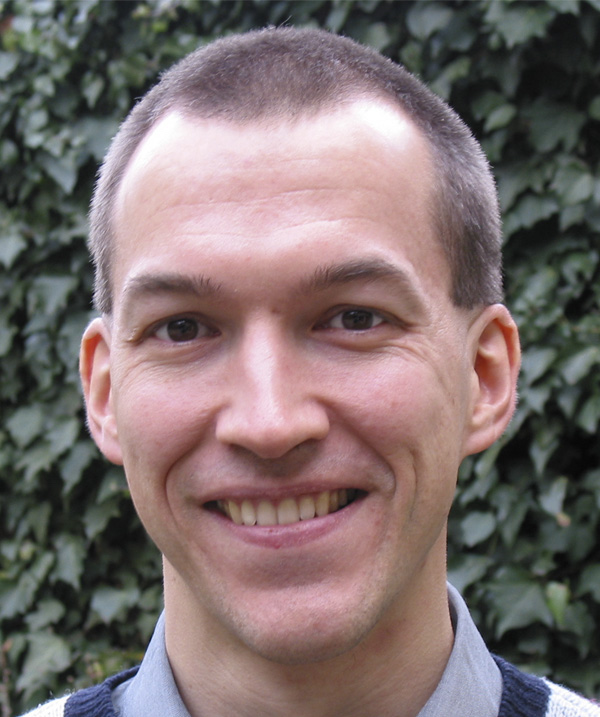
\includegraphics[width=2cm]{figs/tom}
		\hspace{1.6cm}
		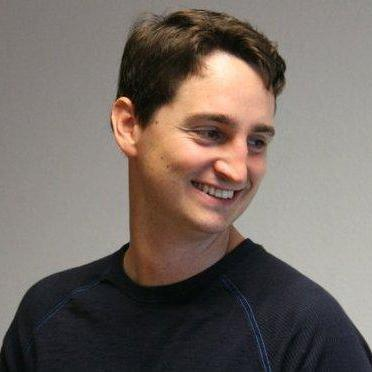
\includegraphics[width=2cm]{figs/grex}    
%        \vspace{0.4cm}
		\\ \hspace{0.4cm} Tom Mens \hspace{1.4cm} Gregorio Robles
		\vspace{0.1cm}
		\\ \hspace{0.8cm} Univ. Mons \hspace{0.8cm} Univ. Rey Juan Carlos
	\end{figure}
\end{center}


\end{frame}

\usebackgroundtemplate{}

%%--------------------------------------------------------

\begin{frame}
\frametitle{Program Committee}

\begin{itemize}
\begin{scriptsize}
  \item Christian Bird, Microsoft Research, USA
  \item Kelly Blincoe, University of Auckland, New Zealand
  \item Jan Bosch, Chalmers University of Technology, Sweden
  \item Marcelo Cataldo, Uber Advanced Technologies Group
  \item Daniel German, University of Victoria, Canada
  \item Matt Germonprez, University of Nebraska Omaha, USA
  \item Sean Goggins, University of Missouri, USA
  \item Jesus Gonzalez-Barahona, Bitergia, Spain
  \item Slinger Jansen, University of Utrecht, Netherlands
  \item Raula Gaikovina Kula, Osaka University, Japan
  \item Josianne Marsan, Laval University, Canada
  \item Wolfgang Mauerer, Siemens/OTH Regensburg, Germany
  \item Alexander Serebrenik, Eindhoven University of Technology, Netherlands
  \item Leif Singer, Automattic, Canada
  \item Margaret-Anne Storey, University of Victoria, Canada
  \item Damian A. Tamburri, Politecnico di Milano, Italy
  \item Bogdan Vasilescu, Carnegie Mellon University, USA
  \item Robert Viseur, University of Mons, Belgium
  \item Stefano Zacchiroli, University of Paris-Diderot, France
  
\end{scriptsize}
\end{itemize}

\end{frame}



%-----------------------    ---------------------------------

\begin{frame}
\frametitle{CHAOSS}

\begin{center}
\begin{figure}[t!]
		
\includegraphics[width=10cm,height=4.6cm]{figs/chaoss}
	\end{figure}
\vspace{-0.2cm}
CHAOSS is a Linux Foundation project focused on creating analytics and metrics to help define community health.\\
https://chaoss.community/
\end{center}


\end{frame}

%-----------------------    ---------------------------------

\begin{frame}
\frametitle{SECOHealth \& SECO-Assist}

\begin{center}
  \begin{columns}[T]

    \begin{column}{0.45\textwidth}
     \begin{block}{SECOHealth}
       \begin{figure}[t!]
         \begin{center}
           
\includegraphics[width=3cm]{figs/secohealth}
         \end{center}
         \label{fig:secohealth}
       \end{figure}
       {\scriptsize Towards an interdisciplinary, socio-technical methodology and analysis of the health of software ecosystems \\ https://secoheal.github.io/}
     \end{block}
    \end{column}
    
    \begin{column}{0.45\textwidth}
      \begin{block}{SECO-Assist}
       \begin{figure}[t!]
          \begin{center}
            
\includegraphics[width=3cm]{figs/seco-assist}
           \end{center}
         \label{fig:secoassist}
       \end{figure}
       \vspace{-0.5cm}
       {\scriptsize Scientific breakthrough to nurture the ecosystems of the future \\ \vspace{0.4cm} https://secoassist.github.io/}
       
     \end{block}
    \end{column}

  \end{columns}
\end{center}

\end{frame}

%%--------------------------------------------------------

\begin{frame}
\frametitle{Today's schedule}

\begin{table}
\centering
\begin{tabular}{l|l}
08:30 - 09:00 &	Opening, registration and coffee \\
09:00 - 09:10 &	Welcome \\
09:10 - 10:30 &	Invited keynote: Kate Stewart \\
10:30 - 11:00 &	Coffee break \\
11:00 - 12:30 &	Session 2: Software Ecosystem Health (4 long) \\
12:30 - 14:00 &	Lunch break \\
14:00 - 14:30 &	Session 3: OSS Health (2 short) \\
14:30 - 15:30 &	Joint CHAOSS/SECOHealth discussion session \\
15:30 - 16:00 &	Coffee break \\
16:00 - 17:15 &	Session 4: Health vs. Cloud, Finances and Global (3 long) \\
17:15 - 17:30 &	Wrap-up \\
\end{tabular}
\end{table}

\vspace{-0.3cm}
\begin{tiny}
Long papers: 13+2 minutes (+15 minutes of discussion after two presentations) \\
\vspace{-0.3cm}
Short presentations: 9+1 minutes (+10 minutes of discussion after two presentations).
\end{tiny}

\end{frame}

%%--------------------------------------------------------

\begin{frame}
\frametitle{Breaking the ice ...}

\begin{figure}[t!]
		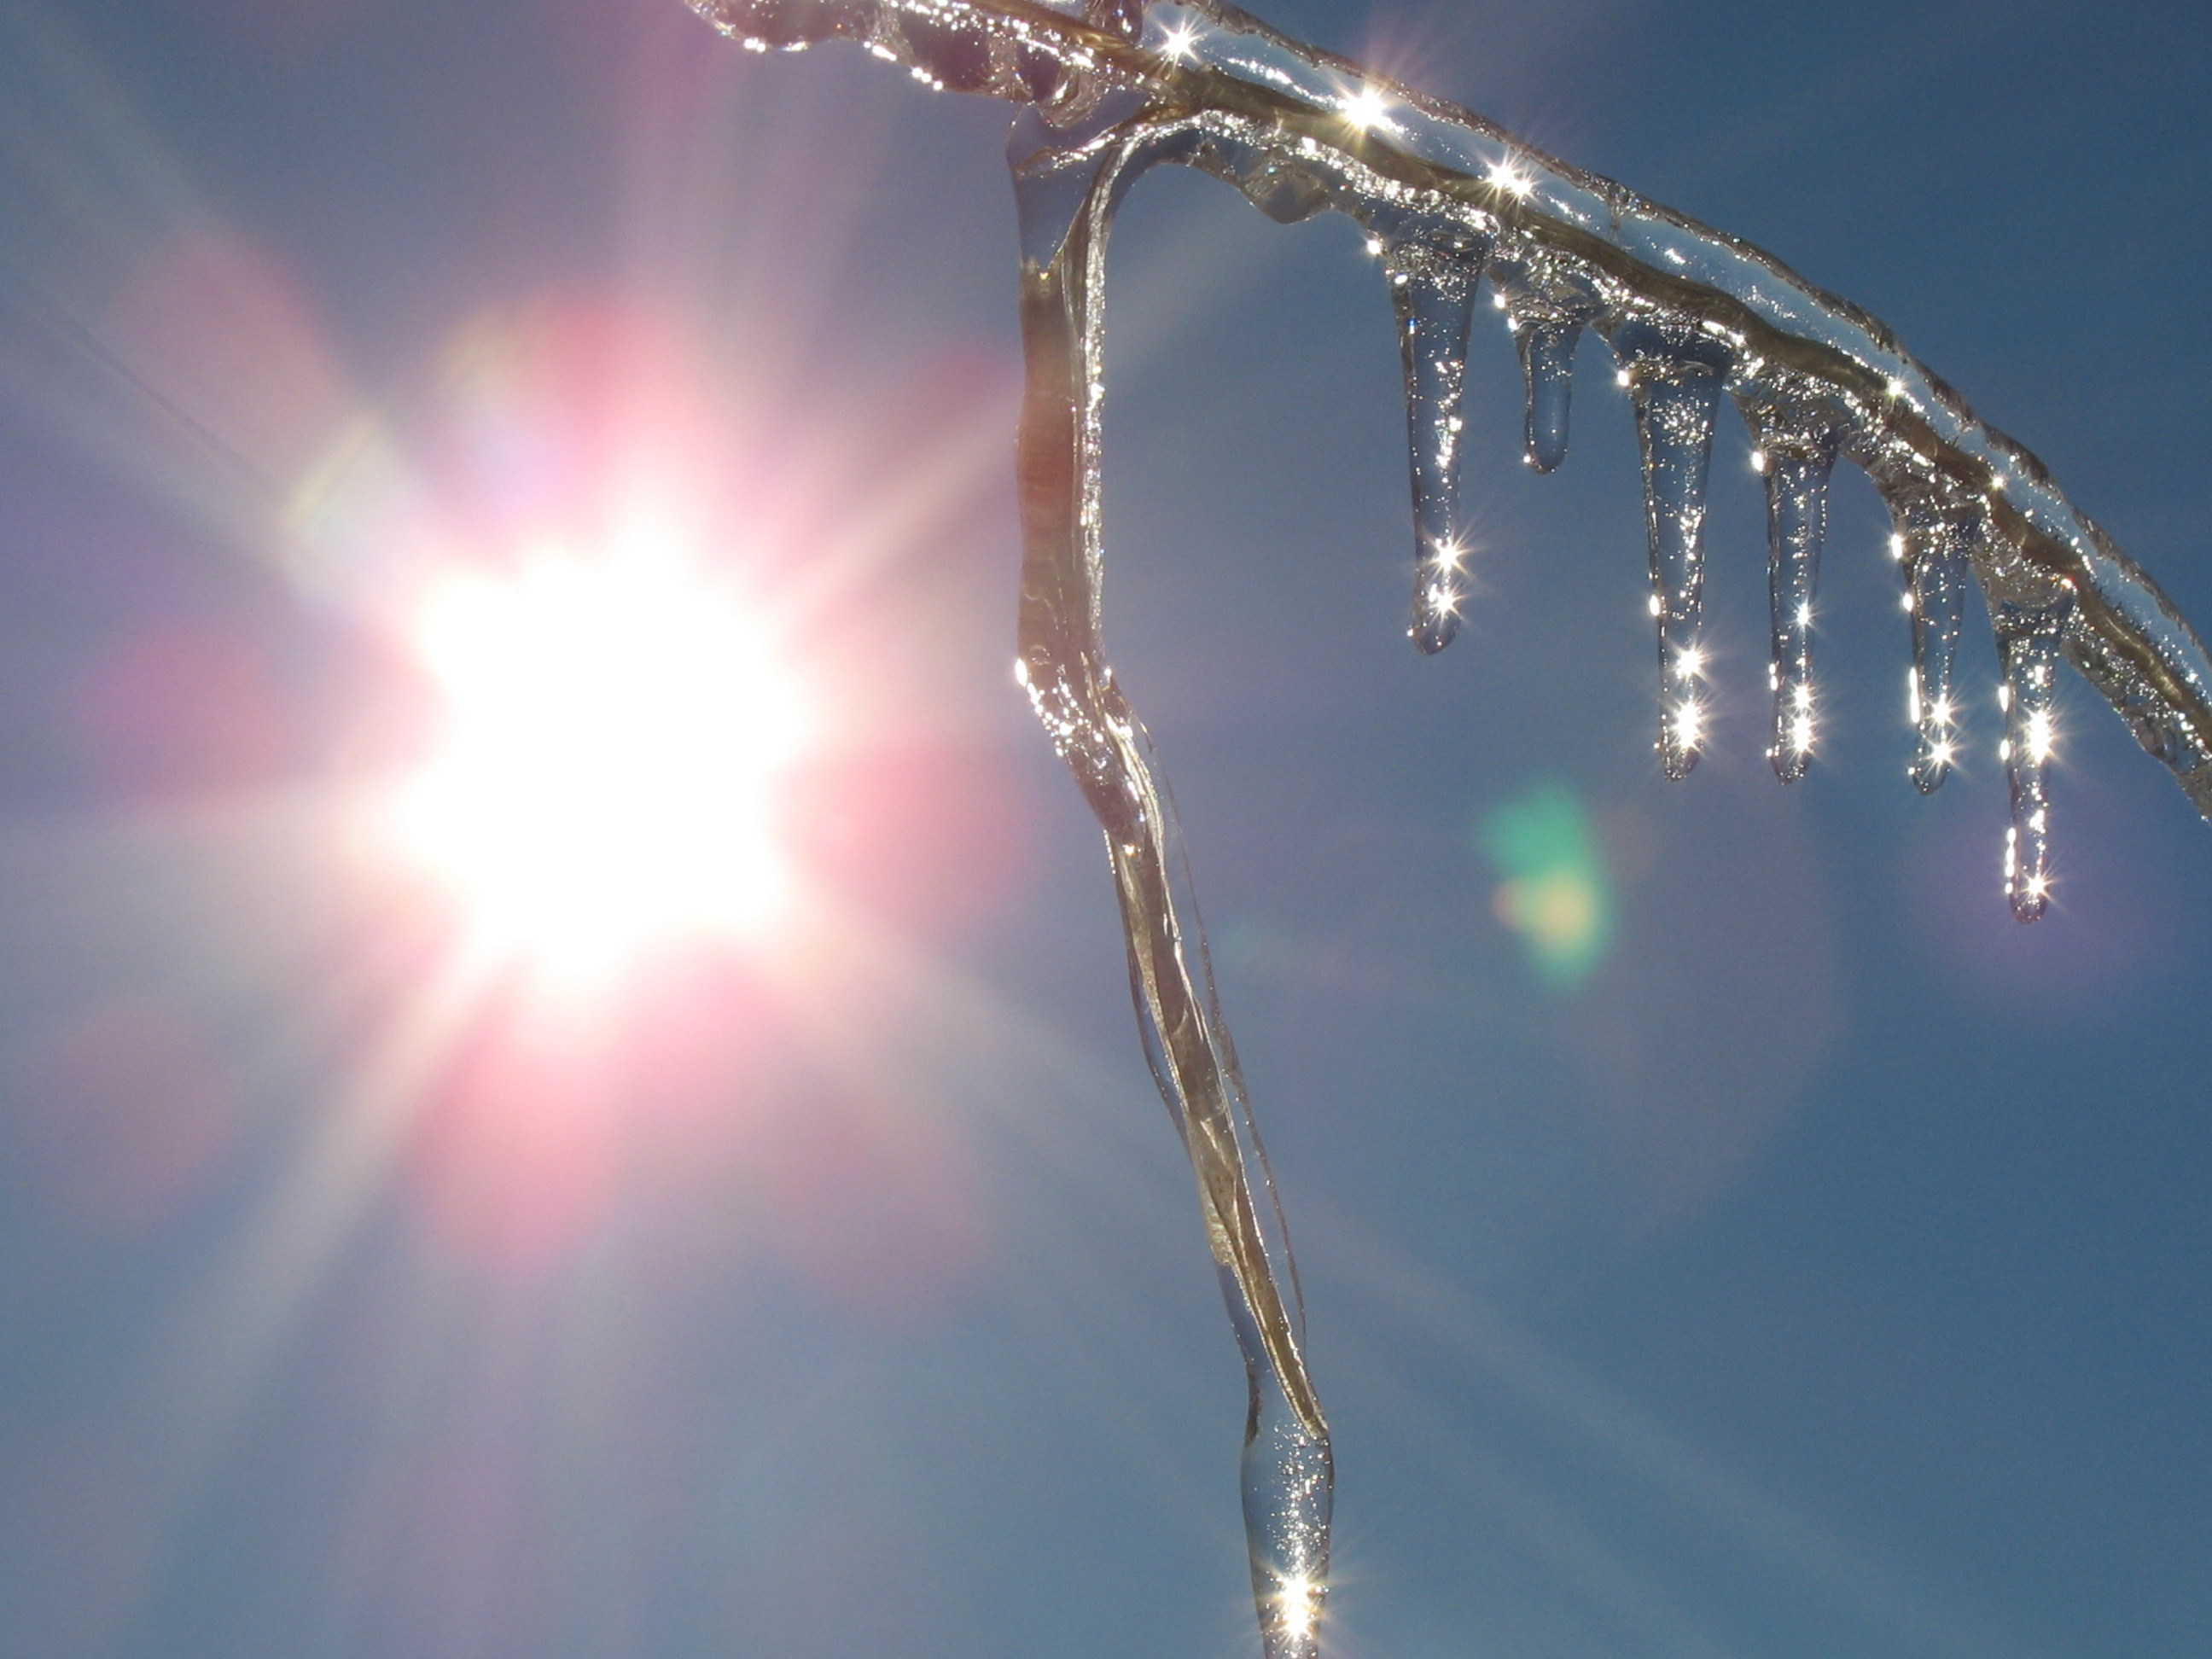
\includegraphics[width=8cm]{figs/ice}
	\end{figure}

Let's introduce each other: who are you and why are you here?

\end{frame}

%-----------------------    ---------------------------------

\begin{frame}
\frametitle{Welcome}

\begin{center}
\Huge Enjoy!
\end{center}


\begin{center}
\Huge \#soheal18
\end{center}

\end{frame}


%-----------------------    ---------------------------------

\begin{frame}
\frametitle{Keynote}

\begin{center}
{\bf Lessons learned from the Linux Kernel:\\ Creating sustained healthy communities} \\
\begin{figure}[t!]
		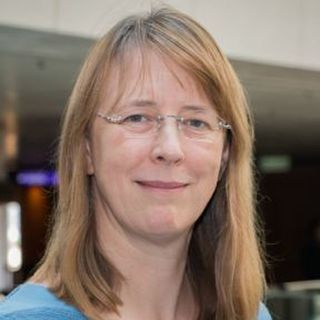
\includegraphics[width=3cm]{figs/kate}
	\end{figure}
\vspace{-0.2cm}
Kate Stewart \\
Linux Foundation \\
Sr. Director of Strategic Programs \\
\end{center}


\end{frame}

\usebackgroundtemplate{}
\end{document}
